% Provenance (never printed): see sources/outline_sources.md (Year 1: the carbonate factory;
% reefs and platforms; pelagic oozes and the carbonate compensation depth; siliceous oozes;
% evaporite sequences). Exercise and problem values in the Book 3 scratch calculator
% calc/ch22.py; figure data from figdata/bachelor-1/evaporation.py and ccd_flank.py.
% Calcite, aragonite and dolomite are ch. 7's; the depth--age law ch. 13's; salinity Book 1's
% (g8); limestone Book 1's (g6, prose); the carbonate system and alkalinity the chemistry and
% biology books' (recalled, never defined). The subsidence of volcanic islands under reefs is
% the Year 2 volume's (oceanic islands); diagenesis (dolomitisation, chert, gypsum to
% anhydrite) is ch. 23's; upwelling ch. 29's.
\chapter{Sedimentos carbonáticos, silicosos e evaporíticos}\label{ch:b1:chemical-biogenic-sediments}

As falésias brancas de giz que se encaram pelo mar estreito entre a Inglaterra e a
França parecem as rochas mais comuns que existem. Ao microscópio eletrônico revelam-se
feitas de incontáveis plaquinhas minúsculas de calcita, deixadas por algas
unicelulares que flutuavam no mar que cobria a região. Um \omterm{def:b1:chemical-biogenic-sediments:reef}{recife} visto de um barco é a
mesma história na outra ponta da escala: um calcário em formação, construído por corais e
algas que retiram cálcio e carbonato da água e os transformam em pedra. Nem todos os
sedimentos são transportados; muitos são formados onde estão, por seres vivos ou pela
própria água ao evaporar. Este capítulo acompanha as três grandes famílias desses
sedimentos --- carbonatos, \omterm{def:b1:chemical-biogenic-sediments:ooze}{lodos silicosos} e \omterm{def:b1:chemical-biogenic-sediments:evaporite}{evaporitos} --- desde a química do mar que
os alimenta até as rochas em que se transformam.

\begin{recall}
O calcário é uma rocha sedimentar feita de calcita, muitas vezes a partir de conchas, e
faz efervescência em ácido diluído (Livro~1, 6º ano). Calcita e aragonita são os dois
\omterm{def:b1:rock-forming-minerals:polymorph}{polimorfos} de \ce{CaCO3}, de densidades \qty{2.71}{g.cm^{-3}} e \qty{2.93}{g.cm^{-3}}, e
a dolomita \ce{CaMg(CO3)2}, de densidade \qty{2.84}{g.cm^{-3}}, é o carbonato de cálcio e
magnésio (\cref{ch:b1:rock-forming-minerals}). A salinidade da água do mar é a massa de
sal dissolvida em um quilograma dela (Livro~1, 8º ano). Na água, o gás carbônico, o íon
hidrogenocarbonato e o íon carbonato estão ligados por equilíbrios ácido-base, e a
alcalinidade mede as bases capazes de captar íons hidrogênio (os livros de química); o
sistema carbonato do oceano participa do ciclo do carbono (os livros de biologia). O
fundo do mar se aprofunda com a idade segundo $d = d_r + C\sqrt t$
(\cref{thm:b1:rifts-ridges-margins:depth-age}).
\end{recall}
% ledger: webmineral:polymorphs, hom:calcite, webmineral:others

\section{A fábrica de carbonatos}\label{sec:b1:chemical-biogenic-sediments:factory}

A água do mar contém cálcio e carbono inorgânico dissolvido, sobretudo como íon
hidrogenocarbonato. Dela se forma o carbonato de cálcio pelas reações
\[
\ce{Ca^2+ + 2 HCO3- -> CaCO3 + CO2 + H2O}, \qquad
\ce{Ca^2+ + CO3^2- -> CaCO3},
\]
a primeira libera uma molécula de gás carbônico para cada carbonato depositado. A água
superficial quente dos trópicos é supersaturada em carbonato de cálcio, mas raramente
precipita por si só: quase tudo é produzido por seres vivos, que pagam a energia para
construir suas conchas e esqueletos e controlam o \omterm{def:b1:rock-forming-minerals:mineral}{mineral} que usam. Corais e algas verdes
constroem aragonita; algas vermelhas e muitos foraminíferos constroem calcita, parte dela
rica em magnésio; os moluscos usam um ou outro.

\begin{definition}[Fábrica de carbonatos]\label{def:b1:chemical-biogenic-sediments:factory}
A \emph{fábrica de carbonatos}\index{fábrica de carbonatos} de um mar é o conjunto de
organismos e processos que produzem sedimento de carbonato de cálcio onde ele é
encontrado, em vez de trazê-lo de outro lugar. Seus produtos são grãos esqueletais
(conchas e esqueletos inteiros ou quebrados), lama carbonática, grãos revestidos e as
estruturas rígidas dos \omterm{def:b1:chemical-biogenic-sediments:reef}{recifes}.
\end{definition}

A fábrica mais rica funciona em águas quentes, claras, rasas e iluminadas pelo sol,
longe da lama dos rios, que enterraria os produtores e turvaria a luz de que as algas
precisam. Seu sedimento é feito pelo próprio fundo do mar: detritos de corais e de
algas, conchas de moluscos e de foraminíferos unicelulares que vivem no fundo, e agulhas
de aragonita deixadas por algas verdes, que se depositam como uma lama calcária. Onde a
água é agitada e supersaturada, os grãos rolados pelas ondas e pelas marés ganham capas
de carbonato, camada sobre camada, em torno de um núcleo, um grão de areia ou um
fragmento de concha, formando \omterm{def:b1:chemical-biogenic-sediments:reef}{oóides} esféricos
(\cref{def:b1:chemical-biogenic-sediments:reef}). Uma segunda fábrica funciona em mar
aberto, longe de qualquer costa: o plâncton que vive na camada superficial iluminada
constrói pequenas conchas e placas de calcita que chovem até o fundo do mar profundo
(\cref{sec:b1:chemical-biogenic-sediments:oozes}).
% ledger: og:carbonates

A velocidade com que uma fábrica constrói é medida pelo seu orçamento de carbonato, a
massa de carbonato produzida e mantida no lugar a cada ano por metro quadrado, depois
das perdas para organismos perfuradores, pastadores e ondas. Ela se transforma em uma
taxa vertical de crescimento por um balanço de massa.

\begin{proposition}[Acreção a partir de um orçamento de carbonato]\label{prop:b1:chemical-biogenic-sediments:accretion}
Seja um fundo marinho que retém a massa líquida $G$ de carbonato de cálcio por unidade
de área e por unidade de tempo, como um depósito cujos grãos sólidos têm densidade
$\rho_s$ e cuja porosidade, a fração de seu volume ocupada por poros, é $\phi$. Então o
fundo se eleva à taxa
\[
a = \frac{G}{\rho_s\,(1-\phi)}.
\]
\end{proposition}

\begin{proof}
No intervalo $\mathrm dt$, uma área unitária recebe a massa $G\,\mathrm dt$ de carbonato
sólido, que preenche o volume $G\,\mathrm dt/\rho_s$ de grãos. Esses grãos formam a
fração $1-\phi$ da nova camada, cuja espessura é, portanto,
$G\,\mathrm dt/(\rho_s(1-\phi))$. Dividindo por $\mathrm dt$ obtém-se $a$.
\end{proof}

O produto $\rho_s(1-\phi)$ é a densidade aparente seca do depósito. Nos \omterm{def:b1:chemical-biogenic-sediments:reef}{recifes} do
arquipélago de Chagos, no oceano Índico, 28 \omterm{def:b1:chemical-biogenic-sediments:reef}{recifes} medidos em 2015 tiveram um orçamento
médio de \qty{3.7}{kg} de \ce{CaCO3} por metro quadrado e por ano, e os dominados por
corais ramificados \emph{Acropora} tiveram \qty{8.4}{kg}, crescendo cerca de
\qty{4.2}{mm} por ano; com a proposição, esses dois números juntos significam uma
densidade aparente seca de \qty{2000}{kg.m^{-3}}, isto é, um arcabouço de \omterm{def:b1:chemical-biogenic-sediments:reef}{recife} com cerca
de um terço de espaço poroso (\cref{exo:b1:chemical-biogenic-sediments:3}). Os mesmos
\omterm{def:b1:chemical-biogenic-sediments:reef}{recifes} tinham perdido mais de nove décimos de seus corais no evento de aquecimento de
1998, e seus orçamentos mostram quão depressa um \omterm{def:b1:chemical-biogenic-sediments:reef}{recife} pode se reconstruir.
% ledger: perry:chagos

\section{Recifes e plataformas}\label{sec:b1:chemical-biogenic-sediments:reefs}

Onde a fábrica constrói um arcabouço rígido, ele pode se erguer do fundo do mar contra
as ondas.

\begin{definition}[Recife, plataforma carbonática, oóide]\label{def:b1:chemical-biogenic-sediments:reef}
Um \emph{recife}\index{recife} é uma construção carbonática cujo arcabouço de organismos,
corais, algas ou outros, crescido no local e ligado e cimentado, se ergue acima do fundo
do mar ao redor e resiste às ondas. Uma \emph{plataforma carbonática}\index{plataforma carbonática} é um corpo espesso de
carbonato de águas rasas, cujo topo plano fica próximo ao nível do mar e que é limitado por um talude descendo até águas mais profundas.
Um \emph{oóide}\index{oóide} é um grão redondo do tamanho de areia, formado por camadas
concêntricas de carbonato de cálcio crescidas em torno de um núcleo enquanto ele rolava
em água agitada; uma rocha feita de oóides é um oólito.
\end{definition}
% ledger: og:carbonates

Os \omterm{def:b1:chemical-biogenic-sediments:reef}{recifes} de coral modernos vêm em três tipos, nomeados pelos viajantes que os mapearam
muito antes de alguém perfurar um deles. Um \omterm{def:b1:chemical-biogenic-sediments:reef}{recife} \emph{franjante} é preso à costa de
uma ilha ou de um continente. Um \omterm{def:b1:chemical-biogenic-sediments:reef}{recife} \emph{barreira} é separado da terra por uma
laguna, que pode ser larga e ter dezenas de metros de profundidade: a barreira ao
nordeste da Austrália se estende, com interrupções, por quase mil milhas (cerca de
\qty{1600}{km}), cercando um mar de 10 a 25 braças de profundidade, cerca de 18 a
\qty{46}{m}. Um \emph{atol} é um anel de \omterm{def:b1:chemical-biogenic-sediments:reef}{recife}, com ilhas baixas de areia de coral, em
torno de uma laguna sem nenhuma terra dentro.

\begin{omfigure}
\begin{tikzpicture}[font=\footnotesize, scale=0.72]
% three reef types in cross-section (schematic): a volcanic cone y = 2 - s - 0.75|x - 4|
% subsided by s (0, 0.8, 1.6), sea level at y = 1; the reef grows up from its first
% position, the foot of the fringing reef at (2, 0.5) moving down with the cone
\foreach \s/\yo/\lab/\name in {0/0/a/recife franjante, 0.8/-3.8/b/recife barreira, 1.6/-7.6/c/atol} {
  \begin{scope}[yshift=\yo cm]
    \begin{scope}
      \clip (0,-1.3) rectangle (8,2.3);
      \fill[omSea] (0,-1.3) rectangle (8,1.0);
      \draw[lith basalt] (-1,2-\s-3.75) -- (4,2-\s) -- (9,2-\s-3.75) -- cycle;
    \end{scope}
    \draw[omSea!60!black] (0,1.0) -- (8,1.0);
    \node[anchor=west, font=\scriptsize] at (8.05,1.0) {nível do mar};
    \node[anchor=west] at (0,2.05) {(\lab) \name};
    \draw[black!70] (1.05,1.55) node[anchor=east, font=\scriptsize] {recife} -- (2.2,1.02);
  \end{scope}
}
% (a) fringing reef: wedges against the shore
\fill[lith reef limestone, draw=black!70] (2.0,0.5) -- (2.15,1.0) -- (2.667,1.0) -- cycle;
\fill[lith reef limestone, draw=black!70] (6.0,0.5) -- (5.85,1.0) -- (5.333,1.0) -- cycle;
\node[anchor=west, font=\scriptsize] at (4.9,1.75) {ilha vulcânica};
% (b) barrier reef: the cone has sunk by 0.8, the reef has grown up, a lagoon opens
\begin{scope}[yshift=-3.8cm]
  \fill[lith reef limestone, draw=black!70] (2.0,-0.3) -- (2.15,1.0) -- (2.6,1.0) -- (2.55,0.1125) -- cycle;
  \fill[lith reef limestone, draw=black!70] (6.0,-0.3) -- (5.85,1.0) -- (5.4,1.0) -- (5.45,0.1125) -- cycle;
  \draw[black!70] (3.2,0.85) -- (3.45,1.55) node[anchor=south west, font=\scriptsize, inner sep=1pt] {laguna};
\end{scope}
% (c) atoll: the cone has sunk by 1.6 and is drowned; the reef ring encloses a lagoon
\begin{scope}[yshift=-7.6cm]
  \fill[lith limestone, draw=black!50] (2.55,-0.6875) -- (2.55,0.55) -- (5.45,0.55) -- (5.45,-0.6875) -- (4,0.4) -- cycle;
  \fill[lith reef limestone, draw=black!70] (2.0,-1.1) -- (2.15,1.0) -- (2.6,1.0) -- (2.55,-0.6875) -- cycle;
  \fill[lith reef limestone, draw=black!70] (6.0,-1.1) -- (5.85,1.0) -- (5.4,1.0) -- (5.45,-0.6875) -- cycle;
  \node[font=\scriptsize] at (4,0.78) {laguna};
  \node[font=\scriptsize, fill=omLithLime, inner sep=1pt] at (4,0.05) {sedimento de laguna};
\end{scope}
% photograph
\node[anchor=north west, inner sep=0] at (10.75,2.3) {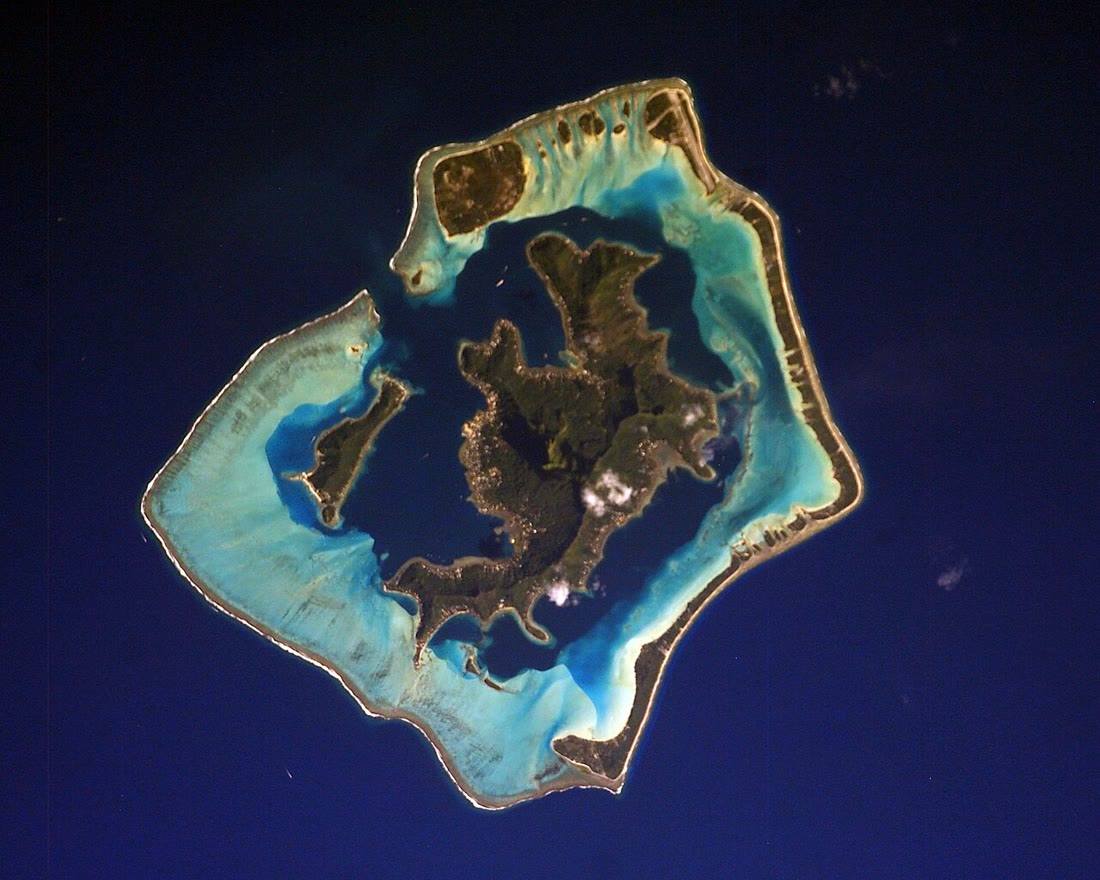
\includegraphics[height=6.9cm]{images/book3/b1-bora-bora.jpg}};
\end{tikzpicture}

{\small À esquerda: os três tipos de \omterm{def:b1:chemical-biogenic-sediments:reef}{recife} de coral em corte transversal (esquemático, com
escala vertical muito exagerada), desenhados como Darwin os explicou: (a)~um \omterm{def:b1:chemical-biogenic-sediments:reef}{recife}
franjando uma ilha vulcânica; (b)~a ilha afundou e o \omterm{def:b1:chemical-biogenic-sediments:reef}{recife}, crescendo para cima, tornou-se
uma barreira separada da costa por uma laguna; (c)~a ilha afundou fora de vista e o \omterm{def:b1:chemical-biogenic-sediments:reef}{recife} é
um atol em torno de uma laguna com sedimento carbonático no fundo. À direita: Bora Bora, uma
ilha vulcânica em uma laguna cercada por um \omterm{def:b1:chemical-biogenic-sediments:reef}{recife} barreira com ilhas baixas sobre ele,
fotografada por um astronauta a partir da Estação Espacial Internacional em 19 de março de
2003 (NASA, domínio público, via Wikimedia Commons).}
\label{fig:b1:chemical-biogenic-sediments:reefs}
\end{omfigure}
% ledger: darwin:reefs, commons:bora-bora

\begin{history}[Recifes sobre fundações que afundam, 1837--1842]
Durante a viagem do \emph{Beagle}, Charles Darwin navegou entre os \omterm{def:b1:chemical-biogenic-sediments:reef}{recifes} dos oceanos
Pacífico e Índico. Ele raciocinou a partir de um fato: corais construtores de \omterm{def:b1:chemical-biogenic-sediments:reef}{recifes},
concluiu, não prosperam, em casos comuns, mais fundo que entre 20 e 30 braças, cerca de
37 a \qty{55}{m}. Entretanto, \omterm{def:b1:chemical-biogenic-sediments:reef}{recifes} barreira e atóis se erguem de águas profundas,
muito abaixo desse limite. Suas fundações, argumentou, devem ter afundado devagar o
bastante para que os corais mantivessem o topo na superfície, crescendo para cima: um
\omterm{def:b1:chemical-biogenic-sediments:reef}{recife} que franjava uma ilha vulcânica torna-se uma barreira à medida que a ilha afunda
dentro dele, e um atol quando a ilha desaparece. Ele leu sua teoria perante a Sociedade
Geológica de Londres em 31 de maio de 1837 e a publicou em 1842 em \emph{The Structure
and Distribution of Coral Reefs}, com um mapa de todos os \omterm{def:b1:chemical-biogenic-sediments:reef}{recifes} do mundo classificados
nos três tipos. Por que as ilhas oceânicas afundam, e até onde, é uma questão do
resfriamento da placa sob elas, tratada no Livro~4.
\end{history}
% ledger: darwin:reefs

Um \omterm{def:b1:chemical-biogenic-sediments:reef}{recife} sobrevive apenas se seu topo permanecer nas águas rasas onde vivem seus
construtores. O nível do mar muda, e a fundação pode subsidir; o que importa é a soma
dos dois, a elevação relativa do nível do mar.

\begin{proposition}[Acompanhar o nível ou afogar-se]\label{prop:b1:chemical-biogenic-sediments:keep-up}
Seja o topo de um \omterm{def:b1:chemical-biogenic-sediments:reef}{recife} situado na profundidade $D_0$ abaixo do nível do mar, que cresce
para cima à taxa $a$, enquanto o nível relativo do mar sobe à taxa $r$, ambas constantes.
Então a profundidade da água sobre o \omterm{def:b1:chemical-biogenic-sediments:reef}{recife} após o tempo $t$ é
\[
D(t) = D_0 + (r - a)\,t .
\]
Se $a \ge r$, o \omterm{def:b1:chemical-biogenic-sediments:reef}{recife} acompanha o mar (quando $a > r$, seu topo chega à superfície e daí
em diante só pode crescer lateralmente); se $a < r$ ele fica para trás, e se seus
construtores não puderem viver mais fundo que $D_{\max}$, ele se afoga após o tempo
$(D_{\max} - D_0)/(r - a)$.
\end{proposition}

\begin{proof}
Meça as alturas para cima a partir de uma marca fixa na fundação. O topo do \omterm{def:b1:chemical-biogenic-sediments:reef}{recife} está em
$h_0 + a t$ e a superfície do mar em $s_0 + r t$, de modo que a profundidade da água sobre
o topo é $D = (s_0 - h_0) + (r - a)t = D_0 + (r-a)t$. Quando $a > r$, $D$ chega a zero em
$t = D_0/(a-r)$ e o \omterm{def:b1:chemical-biogenic-sediments:reef}{recife} não pode crescer acima do mar. Quando $a < r$, $D$ cresce
linearmente e atinge $D_{\max}$ quando $(r-a)t = D_{\max} -
D_0$.
\end{proof}

Um \omterm{def:b1:chemical-biogenic-sediments:reef}{recife} cujo topo se afogou não morre de imediato, mas a luz diminui, os construtores
mudam e a fábrica desacelera, de modo que um \omterm{def:b1:chemical-biogenic-sediments:reef}{recife} que começa a ficar para trás fica
ainda mais para trás: \omterm{def:b1:chemical-biogenic-sediments:reef}{recifes} e plataformas afogados, cobertos por sedimentos de águas
profundas, são encontrados nas encostas de muitas ilhas oceânicas e no registro das rochas.

Ao longo de milhões de anos, as fábricas constroem \omterm{def:b1:chemical-biogenic-sediments:reef}{plataformas carbonáticas}, corpos
espessos de carbonato de águas rasas que crescem à medida que suas fundações subsidem.
Duas formas se repetem (veja a figura abaixo). Uma \emph{plataforma com borda} tem topo
plano, protegido atrás de uma borda de \omterm{def:b1:chemical-biogenic-sediments:reef}{recifes} e de bancos de \omterm{def:b1:chemical-biogenic-sediments:reef}{oóides} em sua margem, que
quebra as ondas; atrás dela fica uma laguna calma de lama calcária, e à frente um talude
íngreme onde blocos e detritos desprendidos da borda caem até a bacia. Uma \emph{rampa}
desce muito suavemente da costa até a bacia, sem quebra: bancos de \omterm{def:b1:chemical-biogenic-sediments:reef}{oóides} e de conchas
onde as ondas agitam o fundo, depois camadas de detritos de conchas varridas por
tempestades, depois lama calcária abaixo do alcance das ondas. Uma plataforma com borda
cresce sobretudo para cima e para fora a partir de sua borda; uma rampa desloca seus
cinturões de sedimento para a costa ou para o mar à medida que o nível do mar sobe ou desce.

\begin{omfigure}
\begin{tikzpicture}[font=\footnotesize, >={Stealth[length=4pt]}]
% (a) rimmed shelf and (b) ramp, schematic cross-sections
\begin{scope}
  \fill[omSea] (0,0.2) rectangle (7.2,2.0);
  \fill[lith limestone, draw=black!60] (0,0) -- (0,1.55) -- (4.3,1.55) -- (4.5,1.75) -- (4.9,1.75) -- (5.1,1.5) -- (6.4,0.35) -- (7.2,0.3) -- (7.2,0) -- cycle;
  \fill[lith reef limestone, draw=black!70] (4.3,1.55) -- (4.5,1.75) -- (4.9,1.75) -- (5.1,1.5) -- (4.8,1.05) -- (4.3,1.05) -- cycle;
  \draw[omSea!60!black] (0,2.0) -- (7.2,2.0);
  \node at (2.1,1.78) {lagoa: lama calcária};
  \node[anchor=south, align=center, font=\scriptsize] at (4.7,2.05) {borda de recifes e\\ bancos de oóides};
  \node[anchor=west, font=\scriptsize] at (5.6,1.2) {talude: detritos};
  \node[font=\scriptsize] at (6.75,0.75) {bacia};
  \node at (3.6,-0.35) {(a) plataforma com borda};
\end{scope}
\begin{scope}[xshift=8.0cm]
  \fill[omSea] (0,0.2) rectangle (7.2,2.0);
  \fill[lith limestone, draw=black!60] (0,0) -- (0,1.85) -- (7.2,0.55) -- (7.2,0) -- cycle;
  \draw[omSea!60!black] (0,2.0) -- (7.2,2.0);
  \draw[densely dashed, black!50] (0,1.6) -- (7.2,1.6) node[pos=1, anchor=south east, font=\scriptsize, inner sep=1pt] {ondas de bom tempo alcançam};
  \draw[densely dashed, black!50] (0,1.0) -- (7.2,1.0) node[pos=1, anchor=south east, font=\scriptsize, inner sep=1pt] {ondas de tempestade alcançam};
  \node[anchor=south, font=\scriptsize] at (0.9,2.05) {bancos de oóides};
  \node[anchor=south, font=\scriptsize] at (3.4,2.05) {leitos de conchas de tempestade};
  \node[anchor=south, font=\scriptsize] at (6.1,2.05) {lama calcária};
  \node at (3.6,-0.35) {(b) rampa};
\end{scope}
\end{tikzpicture}

{\small O par de formas de \omterm{def:b1:chemical-biogenic-sediments:reef}{plataforma carbonática} (esquemático, taludes muito exagerados).
(a)~Uma plataforma com borda: uma borda de \omterm{def:b1:chemical-biogenic-sediments:reef}{recifes} e bancos de \omterm{def:b1:chemical-biogenic-sediments:reef}{oóides} quebra as ondas, uma
laguna calma de lama calcária fica atrás dela, e detritos desprendidos da borda descem pelo
talude até a bacia. (b)~Uma rampa desce suavemente da costa até a bacia, seus sedimentos
separados pela profundidade que as ondas alcançam.}
\label{fig:b1:chemical-biogenic-sediments:platforms}
\end{omfigure}

\section{Lodos pelágicos e a profundidade de compensação do carbonato}\label{sec:b1:chemical-biogenic-sediments:oozes}

Longe da terra, o fundo do mar recebe quase nada dos continentes além da poeira mais fina
trazida pelo vento. O que nele cai são os esqueletos do plâncton que vivia na água
iluminada, quilômetros acima: as placas de calcita dos cocolitoforídeos e as conchas dos
foraminíferos, as frústulas de opala das diatomáceas e os esqueletos dos radiolários
(fotografados um pouco adiante). A longa chuva de cocolitos até o fundo do mar é o
principal processo que forma o giz e grande parte do calcário do mundo.
% ledger: nasa:coccoliths-b3, og:carbonates

\begin{definition}[Lodo calcário, lodo silicoso]\label{def:b1:chemical-biogenic-sediments:ooze}
Um lodo é um sedimento pelágico de granulometria fina, depositado em mar aberto e formado
sobretudo pelos esqueletos do plâncton. É um \emph{lodo calcário}\index{lodo calcário}
quando eles são de carbonato de cálcio, sobretudo cocolitos e foraminíferos, e um
\emph{lodo silicoso}\index{lodo silicoso} quando são de opala, sílica amorfa hidratada,
sobretudo diatomáceas e radiolários.
\end{definition}
% ledger: og:carbonates

Os \omterm{def:b1:chemical-biogenic-sediments:ooze}{lodos calcários} cobrem cerca de metade do fundo do mar do mundo, mas só acima de certa
profundidade: abaixo de cerca de \qty{4500}{m} eles desaparecem. As conchas não deixam de
cair ali; elas se dissolvem. O oceano profundo é frio e a pressão é alta, e a solubilidade
da calcita aumenta com a profundidade, sobretudo por causa da pressão, enquanto a
concentração de íon carbonato na água geralmente diminui com a profundidade (a química
desses equilíbrios é recordada dos livros de química). Abaixo de certa profundidade a água
profunda é subsaturada em calcita, e as conchas que chegam ao fundo se dissolvem tanto
mais depressa quanto mais fundo jazem.
% ledger: britannica:ccd, slotnick:ccd-definitions

\begin{omfigure}
\begin{tikzpicture}
\node[inner sep=0] (a) at (0,0) {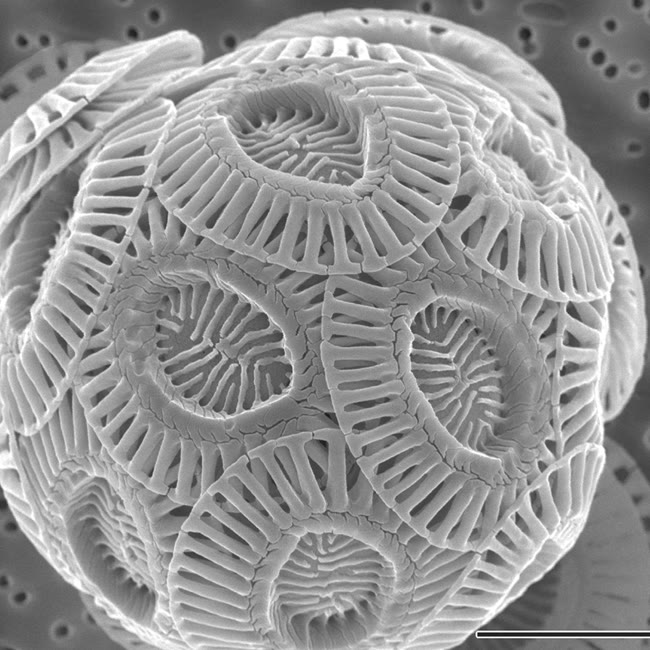
\includegraphics[height=4.3cm]{images/book3/b1-coccolithophore.jpg}};
\node[inner sep=0, anchor=west] (b) at ([xshift=0.25cm]a.east) {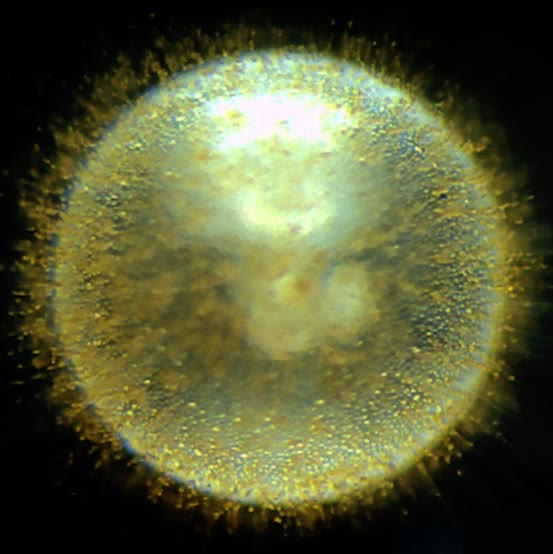
\includegraphics[height=4.3cm]{images/book3/b1-orbulina.jpg}};
\node[inner sep=0, anchor=west] (c) at ([xshift=0.25cm]b.east) {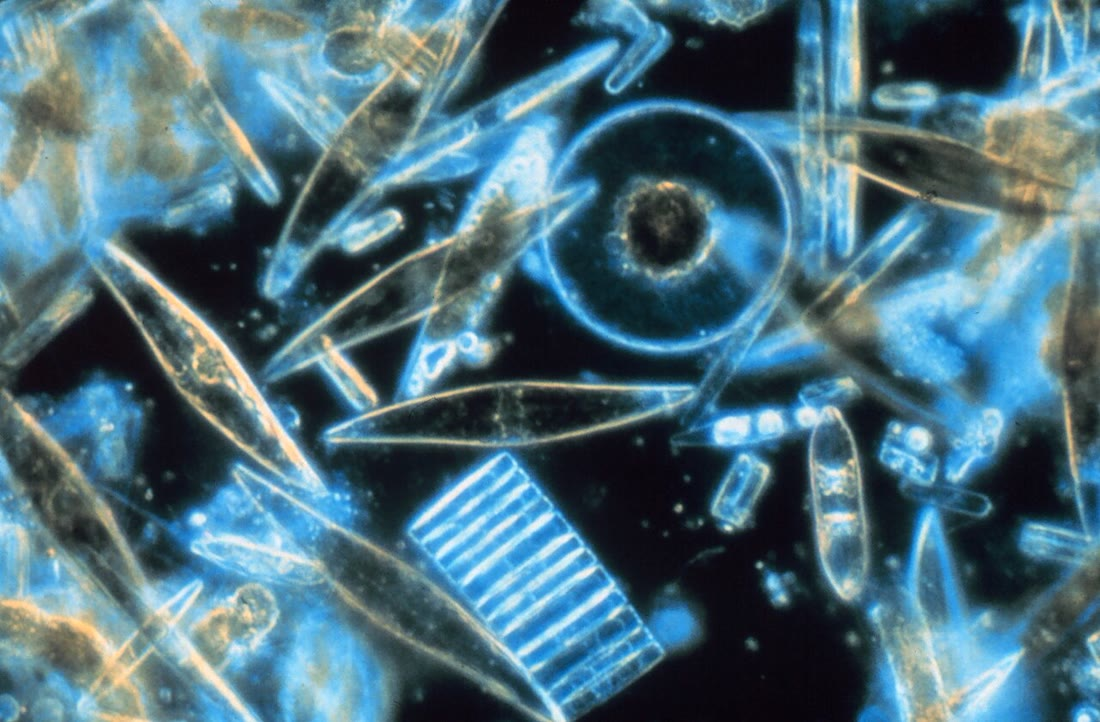
\includegraphics[height=4.3cm]{images/book3/b1-diatoms.jpg}};
  \node[font=\footnotesize, anchor=north] at (a.south) {(a) um cocolitoforídeo};
  \node[font=\footnotesize, anchor=north] at (b.south) {(b) um foraminífero};
  \node[font=\footnotesize, anchor=north] at (c.south) {(c) diatomáceas};
\end{tikzpicture}

{\small Os produtores de lodos. (a)~Uma única célula de \emph{Emiliania huxleyi}, revestida
de cocolitos, com suas placas de calcita (microscópio eletrônico de varredura; Alison
R.~Taylor, University of North Carolina Wilmington, CC~BY~2.5, via Wikimedia Commons).
(b)~Um foraminífero planctônico vivo, \emph{Orbulina universa}, com sua concha de calcita
cercada de espinhos (microscópio de luz; H.~Takagi e coautores, 2019, CC~BY~4.0, via
Wikimedia Commons). (c)~Diatomáceas vivas do gelo marinho do Estreito de McMurdo,
Antártida, cada uma em sua frústula de opala (microscópio de luz; Gordon T.~Taylor, Stony
Brook University, NOAA, domínio público, via Wikimedia Commons).}
\label{fig:b1:chemical-biogenic-sediments:plankton}
\end{omfigure}
% ledger: commons:ehux, commons:orbulina, commons:diatoms-noaa

\begin{definition}[Lisoclina, profundidade de compensação do carbonato]\label{def:b1:chemical-biogenic-sediments:ccd}
A \emph{lisoclina}\index{lisoclina} é a profundidade no oceano abaixo da qual a dissolução
da calcita no fundo do mar aparece primeiro no sedimento e sua taxa aumenta bruscamente.
A \emph{profundidade de compensação do carbonato}\index{profundidade de compensação do carbonato}
(CCD) é a profundidade em que a taxa de dissolução da calcita iguala a taxa com que a calcita
chove sobre o fundo do mar; abaixo dela nenhum carbonato de cálcio se acumula. Na prática
ela é situada onde o teor de carbonato de cálcio do sedimento superficial cai abaixo de
\qty{10}{\%} em peso.
\end{definition}
% ledger: slotnick:ccd-definitions

A CCD fica em geral centenas de metros abaixo da \omterm{def:b1:chemical-biogenic-sediments:ccd}{lisoclina}. Ela não é um nível fixo: é
definida por um equilíbrio entre suprimento e dissolução, de modo que fica mais fundo onde
o plâncton produz mais carbonato e onde a água profunda é menos corrosiva. No Atlântico ela
fica cerca de \qty{500}{m} mais fundo que no Pacífico, resultado de um suprimento maior de
carbonato e de uma dissolução mais lenta; no Pacífico ocidental, ela fica a cerca de
\qty{4000}{m} no noroeste e a cerca de \qty{5100}{m} no Pacífico central. A aragonita, mais
solúvel que a calcita, se dissolve em profundidades ainda menores. Ao longo do tempo
geológico, mudanças no suprimento, na produtividade e na dissolução deslocaram a CCD em
mais de \qty{2000}{m}.
% ledger: slotnick:ccd-definitions, britannica:ccd, zhang:ccd-west-pacific

\begin{method}[Localizando a lisoclina e a CCD]\label{met:b1:chemical-biogenic-sediments:ccd}
\begin{enumerate}
  \item Colete os primeiros centímetros de sedimento em pontos de profundidades diferentes
        em uma mesma região, longe o bastante da terra e da ressurgência para que a diluição
        por argila ou por opala seja pequena.
  \item Meça a porcentagem em peso de \ce{CaCO3} de cada amostra e plote-a contra a
        profundidade da água.
  \item A \omterm{def:b1:chemical-biogenic-sediments:ccd}{lisoclina} é a profundidade onde o teor começa a cair bruscamente, e onde as conchas
        mostram os primeiros sinais de dissolução (foraminíferos quebrados, corroídos).
  \item A CCD é a profundidade em que o teor cai para \qty{10}{\%}: leia-a por interpolação
        linear entre as duas amostras de cada lado.
\end{enumerate}
\end{method}

Na encosta de uma dorsal meso-oceânica, o fundo do mar é jovem e raso perto do eixo e afunda
à medida que envelhece e se afasta. Um pedaço de fundo nascido acima da CCD acumula \omterm{def:b1:chemical-biogenic-sediments:ooze}{lodo
calcário} até afundar abaixo da CCD; daí em diante recebe apenas o que não se dissolve: a
poeira que se assenta do ar, óxidos de ferro e manganês, dentes de peixes. Esse depósito
lento e marrom é a argila vermelha das bacias profundas.

\begin{proposition}[Cruzando a CCD]\label{prop:b1:chemical-biogenic-sediments:flank}
Seja o fundo do mar de idade $t$ situado na profundidade $d(t) = d_r + C\sqrt t$
(\cref{thm:b1:rifts-ridges-margins:depth-age}), com o eixo de uma dorsal na profundidade
$d_r$ mais rasa que uma \omterm{def:b1:chemical-biogenic-sediments:ccd}{profundidade de compensação do carbonato} $z_c$ que permanece
constante. Então o fundo passa abaixo da CCD na idade
\[
t_c = \left(\frac{z_c - d_r}{C}\right)^2 ,
\]
e um local de idade $t > t_c$ carrega, de baixo para cima, a \omterm{def:b1:layered-earth:layers}{crosta} vulcânica, o \omterm{def:b1:chemical-biogenic-sediments:ooze}{lodo
calcário} depositado durante o tempo $t_c$ e a argila vermelha depositada durante o tempo
$t - t_c$.
\end{proposition}

\begin{proof}
A profundidade $d(t)$ cresce com $t$, e $d(t_c) = z_c$ dá $C\sqrt{t_c} =
z_c - d_r$, daí
$t_c$. Antes de $t_c$ o fundo fica acima da CCD, onde a calcita chove mais depressa do que
se dissolve e o lodo se acumula; depois de $t_c$ ele fica abaixo, onde nenhum carbonato se
acumula e só a argila insolúvel é acrescentada. O lodo, uma vez soterrado sob a argila,
fica protegido da água corrosiva de cima, de modo que a ordem das camadas é a dos tempos.
\end{proof}

Com $d = 2500 + 350\sqrt t$ (metros, $t$ em milhões de anos), uma CCD a \qty{4500}{m} é
cruzada na idade $(2000/350)^2 = \qty{32.7}{Myr}$; a uma taxa de meia-expansão de
\qty{25}{mm} por ano, isso dá \qty{816}{km} do eixo (figura abaixo). A perfuração em fundo
oceânico antigo
encontra essa ordem repetidas vezes: basalto, depois \omterm{def:b1:chemical-biogenic-sediments:ooze}{lodo calcário} ou giz, depois argila
vermelha, um registro da jornada do fundo pela encosta abaixo. Onde a placa se deslocou
depois sob um cinturão de alta produtividade, perto do equador, a argila pode ser coberta
por uma nova camada de lodo, e é assim que os testemunhos registram o movimento das placas
além da profundidade da CCD.
% ledger: parsons:plate-model

\begin{omfigure}
\begin{tikzpicture}[font=\footnotesize]
\begin{axis}[width=11cm, height=5.6cm, xmin=0, xmax=1750, ymin=2000, ymax=6200, y dir=reverse,
  xlabel={distância do eixo da dorsal (km), taxa de meia-expansão \qty{25}{mm.yr^{-1}}},
  ylabel={profundidade (m)}, ytick={2000,3000,...,6000},
    axis on top, clip=false]
  % sea water above the floor
  \addplot[fill=omSea, draw=none] table[x=x_km, y=depth] {figdata/out/bachelor-1-ccd_flank-profile.dat} -- (axis cs:1750,2000) -- (axis cs:0,2000) -- cycle;
  % floor: ooze-covered above the CCD, red clay below
  \addplot[very thick, draw=omLithLime!70!black, restrict x to domain=0:816.3] table[x=x_km, y=depth] {figdata/out/bachelor-1-ccd_flank-profile.dat};
  \addplot[very thick, draw=brown!70!black, restrict x to domain=816.3:1750] table[x=x_km, y=depth] {figdata/out/bachelor-1-ccd_flank-profile.dat};
  \draw[thick, omThm, densely dashed] (axis cs:0,4500) -- (axis cs:1750,4500) node[pos=0.99, anchor=north east, inner sep=1.5pt] {CCD, \qty{4500}{m}};
  \draw[black!60, dotted, thick] (axis cs:0,4050) -- (axis cs:1750,4050) node[pos=0.99, anchor=south east, inner sep=1.5pt] {lisoclina (esquemática)};
  \fill[omThm] (axis cs:816.3,4500) circle[radius=2pt];
  \node[anchor=north east, align=right] at (axis cs:790,4620) {o fundo cruza a CCD\\ a \qty{32.7}{Myr}, \qty{816}{km}};
  \node[anchor=north, align=center, omLithLime!40!black] at (axis cs:520,2750) {lodo calcário\\ se acumula};
  \node[anchor=north west, align=left, brown!60!black] at (axis cs:1000,5180) {argila vermelha sobre\\ lodo soterrado};
\end{axis}
% sediment column at the site 1500 km from the axis (60 Myr), schematic
\begin{scope}[xshift=10.6cm, yshift=0.4cm]
  \draw[lith basalt] (0,0) rectangle (0.9,1.0);
  \draw[lith limestone] (0,1.0) rectangle (0.9,2.6);
  \fill[brown!45, draw=black!60] (0,2.6) rectangle (0.9,3.2);
  \node[anchor=west, align=left, font=\scriptsize] at (1.0,0.5) {crosta basáltica};
  \node[anchor=west, align=left, font=\scriptsize] at (1.0,1.8) {lodo calcário\\ (0 a \qty{32.7}{Myr})};
  \node[anchor=west, align=left, font=\scriptsize] at (1.0,2.9) {argila vermelha};
  \node[anchor=south, font=\scriptsize, align=center] at (0.9,3.3) {coluna a \qty{1500}{km}\\ (esquemática)};
\end{scope}
\end{tikzpicture}

{\small Sedimentos pelágicos em uma encosta de dorsal. O fundo se aprofunda com a idade
pela \omterm{thm:b1:rifts-ridges-margins:depth-age}{lei profundidade--idade} $d = 2500 + 350\sqrt t$ e se afasta do eixo a \qty{25}{mm} por
ano; acima da \omterm{def:b1:chemical-biogenic-sediments:ccd}{profundidade de compensação do carbonato}, tomada aqui a \qty{4500}{m}, ele
acumula \omterm{def:b1:chemical-biogenic-sediments:ooze}{lodo calcário}, e abaixo dela apenas argila vermelha. Um local distante do eixo
carrega basalto, lodo e argila vermelha, de baixo para cima (coluna à direita, espessuras
esquemáticas). A \omterm{def:b1:chemical-biogenic-sediments:ccd}{lisoclina}, desenhada algumas centenas de metros acima da CCD, marca onde
a dissolução começa a aparecer.}
\label{fig:b1:chemical-biogenic-sediments:flank}
\end{omfigure}
% computed in figdata/bachelor-1/ccd_flank.py; ledger: parsons:plate-model, britannica:ccd, slotnick:ccd-definitions

\section{Lodos silicosos e cherts}\label{sec:b1:chemical-biogenic-sediments:silica}

Diatomáceas, algas unicelulares do plâncton, e radiolários, membros unicelulares do
zooplâncton, constroem seus esqueletos de opala, que retiram do ácido silícico dissolvido
na água do mar. Ao contrário da calcita da superfície do oceano, a opala não é protegida
pela supersaturação: a água do mar é subsaturada nela em todas as profundidades, e a maior
parte da opala se dissolve assim que o organismo morre, primeiro na água enquanto afunda e
depois no fundo do mar. Dos 255~teramoles de silício incorporados à opala a cada ano pelo
plâncton do oceano mundial, apenas cerca de 9.2 ficam soterrados no sedimento para sempre:
uma preservação de \qty{3.6}{\%}. Um átomo de silício trazido ao mar por um rio é absorvido
e liberado de novo pelo plâncton cerca de dezesseis vezes antes de ser soterrado, e
permanece cerca de \num{8000} anos no oceano.
% ledger: treguer:silica

Assim, \omterm{def:b1:chemical-biogenic-sediments:ooze}{lodos silicosos} se formam onde a produção de opala é tão alta que mesmo
\qty{3.6}{\%} dela se acumula, e onde pouca coisa mais os dilui: em torno do oceano
Antártico, no Pacífico norte, ao longo do equador no Pacífico e nas margens continentais,
os lugares onde a água profunda rica em nutrientes sobe à superfície
(\cref{ch:b1:ocean-circulation}). Eles também dominam abaixo da CCD sob águas produtivas,
onde a calcita que caiu junto com eles se dissolveu.
% ledger: treguer:silica, og:carbonates

\begin{definition}[Sílex]\label{def:b1:chemical-biogenic-sediments:chert}
Um \emph{chert}\index{chert} é uma rocha sedimentar dura e densa de quartzo
microcristalino, formada na maioria dos casos a partir de opala biogênica que se dissolveu
e recristalizou após o soterramento; ocorre em camadas, muitas vezes a partir de \omterm{def:b1:chemical-biogenic-sediments:ooze}{lodos
silicosos}, ou em nódulos, dos quais o sílex, no giz, é o mais conhecido.
\end{definition}
% ledger: og:carbonates

Um lodo de diatomáceas que não foi recristalizado torna-se diatomito, uma rocha clara,
branca e porosa, quase opala pura. Com o soterramento e o tempo, a opala se transforma em
outras formas de sílica e, por fim, em quartzo, e a sílica migra: deixa o giz, por exemplo,
e se concentra em nódulos de sílex ao longo de certas camadas. Como isso acontece pertence
à diagênese (\cref{ch:b1:diagenesis-basins}).

\section{Evaporitos}\label{sec:b1:chemical-biogenic-sediments:evaporites}

Onde uma massa de água do mar perde mais água por evaporação do que recebe, seus sais se
concentram até precipitarem um após o outro. A composição da água do mar é a mesma, em
seus íons principais, em todos os oceanos (\cref{tab:b1:chemical-biogenic-sediments:seawater}).

\begin{table}[htbp]
\centering\small
\begin{tabular}{@{}lrrr@{}}
\hline
íon & fração em massa do sal marinho & \si{g} por \si{kg} de água do mar & \si{mmol} por \si{kg} \\
\hline
cloreto \ce{Cl-} & 0.5503 & 19.353 & 545.9 \\
sódio \ce{Na+} & 0.3066 & 10.781 & 469.0 \\
sulfato \ce{SO4^2-} & 0.0771 & 2.712 & 28.2 \\
magnésio \ce{Mg^2+} & 0.0365 & 1.284 & 52.8 \\
cálcio \ce{Ca^2+} & 0.0117 & 0.412 & 10.3 \\
potássio \ce{K+} & 0.0113 & 0.399 & 10.2 \\
hidrogenocarbonato \ce{HCO3-} & 0.0030 & 0.105 & 1.72 \\
brometo \ce{Br-} & 0.0019 & 0.067 & 0.84 \\
\hline
todos os solutos & 1 & 35.165 & \\
\hline
\end{tabular}
\caption{Os íons principais da água do mar de composição de referência, para uma salinidade
de \qty{35.165}{g} de sal por quilograma de água do mar. Cloreto e sódio formam
\qty{86}{\%} do sal em massa; carbonato, estrôncio, borato e fluoreto formam a maior parte
do restante.}
\label{tab:b1:chemical-biogenic-sediments:seawater}
\end{table}
% ledger: teos10:reference-composition, teos10:reference-salinity (g and mmol computed in evaporation.py)

\begin{definition}[Evaporito, sequência de evaporação, sabkha]\label{def:b1:chemical-biogenic-sediments:evaporite}
Um \emph{evaporito}\index{evaporito} é um sedimento ou rocha sedimentar de sais precipitados
de uma salmoura natural concentrada por evaporação: sobretudo gipsita \ce{CaSO4.2H2O} e
anidrita \ce{CaSO4}, halita \ce{NaCl}, e os sais de potássio e magnésio. A
\emph{sequência de evaporação}\index{sequência de evaporação} é a ordem em que os \omterm{def:b1:rock-forming-minerals:mineral}{minerais}
precipitam da água do mar em evaporação, o menos solúvel primeiro: carbonato de cálcio,
depois gipsita, depois halita, depois os sais de potássio e magnésio. Uma
\emph{sabkha}\index{sabkha} é uma salina costeira, no nível ou logo acima do nível das marés
mais altas, onde gipsita, anidrita e halita crescem dentro do sedimento a partir da salmoura
em evaporação que o embebe.
\end{definition}
% ledger: og:carbonates, warren:brine-stages

A sequência foi observada já em 1849 por Usiglio, que evaporou um recipiente de água do
mar até secar; as medições mais precisas vêm das salinas de Great Inagua, nas Bahamas,
onde a água do mar é conduzida por uma série de tanques de concentração crescente. O
carbonato de cálcio começa a precipitar quando a salmoura está 1.8~vezes mais concentrada
que a água do mar, a gipsita a 3.8~vezes, a halita a 10.6~vezes; em laboratório, o sulfato
de magnésio segue a cerca de 70~vezes e os sais de potássio acima de 90~vezes. Como os
sais precipitados antes são uma parte desprezível da massa, um fator de concentração de
10.6 significa que resta $1/10.6$, cerca de \qty{9}{\%}, da água: a halita aparece só quando
nove décimos da água já saíram (figura abaixo, painel~a). A salmoura fica mais densa à
medida que se concentra, de \qty{1.03}{g.cm^{-3}} na água do mar para cerca de \num{1.13}
quando a gipsita se forma, \num{1.22} com a halita e mais de \num{1.30} com os sais
amargos, os últimos de todos.
% ledger: warren:brine-stages, mccaffrey:thresholds

Quanto de cada sal um quilograma de água do mar pode fornecer decorre da tabela
\cref{tab:b1:chemical-biogenic-sediments:seawater} ao contar o íon que se esgota primeiro.
O carbonato de cálcio é limitado pelo carbonato e pelo hidrogenocarbonato, \qty{1.10}{mmol},
cerca de \qty{0.11}{g}. A gipsita toma o cálcio restante, \qty{9.18}{mmol}, \qty{1.58}{g},
com o sulfato em excesso. A halita toma todo o sódio, \qty{469}{mmol}, \qty{27.4}{g}, com o
cloreto em excesso. O que sobra, cerca de \qty{6.3}{g} de magnésio, potássio, sulfato,
cloreto e brometo, forma os sais amargos. A halita é \qty{78}{\%} do total: uma bacia de
\omterm{def:b1:chemical-biogenic-sediments:evaporite}{evaporitos} seca é, acima de tudo, uma massa de sal-gema.
% computed in figdata/bachelor-1/evaporation.py; ledger: teos10:reference-composition, mccaffrey:thresholds

\begin{omfigure}
\begin{tikzpicture}[font=\footnotesize]
\begin{axis}[name=a, width=7.6cm, height=5.6cm, xmode=log, xmin=1, xmax=100, ymin=0, ymax=1.05,
  xlabel={fator de concentração da salmoura}, ylabel={fração da água que resta},
  title={\footnotesize (a) início da sequência de evaporação}, grid=major, grid style={black!10},
    log ticks with fixed point]
  \addplot[omDef, thick] table[x=CF, y=f_left] {figdata/out/bachelor-1-evaporation-curve.dat};
  \addplot[omThm, only marks, mark=*, mark size=1.8pt] table[x=CF, y=f_left] {figdata/out/bachelor-1-evaporation-steps.dat};
  \node[anchor=south west, font=\scriptsize] at (axis cs:1.8,0.556) {\ce{CaCO3} (1.8)};
  \node[anchor=south west, font=\scriptsize] at (axis cs:3.8,0.263) {gipsita (3.8)};
  \node[anchor=south west, font=\scriptsize] at (axis cs:10.6,0.094) {halita (10.6)};
  \node[anchor=south, font=\scriptsize, align=center] at (axis cs:60,0.16) {sais de Mg e K\\ (70, 90)};
\end{axis}
\begin{axis}[at={(a.east)}, anchor=west, xshift=1.7cm, width=7.0cm, height=5.6cm,
    ybar, bar width=14pt, ymin=0, ymax=32, xmin=0.4, xmax=4.6,
    xtick={1,2,3,4}, xticklabels={\ce{CaCO3}, gipsita, halita, sais amargos},
    ylabel={gramas por kg de água do mar}, title={\footnotesize (b) massas depositadas},
    nodes near coords, nodes near coords style={font=\scriptsize, /pgf/number format/precision=2},
    every node near coord/.append style={/pgf/number format/fixed}]
  \addplot[fill=omDef!40, draw=omDef] table[x=idx, y=g_per_kg] {figdata/out/bachelor-1-evaporation-masses.dat};
\end{axis}
\end{tikzpicture}

{\small A evaporação da água do mar. (a)~A fração da água que resta quando a salmoura é
concentrada por um dado fator, com o início de cada \omterm{def:b1:rock-forming-minerals:mineral}{mineral} medido nas salinas de Great
Inagua e em laboratório (McCaffrey, Lazar e Holland, 1987). (b)~As massas depositadas por
quilograma de água do mar evaporada até secar, cada \omterm{def:b1:rock-forming-minerals:mineral}{mineral} tomando todo o íon que o
limita (a gipsita contada com sua água; os sais amargos contados sem a sua), calculadas a
partir da composição de referência da água do mar.}
\label{fig:b1:chemical-biogenic-sediments:evaporation}
\end{omfigure}
% computed in figdata/bachelor-1/evaporation.py; ledger: mccaffrey:thresholds, teos10:reference-composition

A partir dessas massas, a espessura de sal que um dado corpo de água pode deixar segue de
imediato.

\begin{proposition}[Sal a partir de uma coluna de água do mar]\label{prop:b1:chemical-biogenic-sediments:column}
Uma coluna de água do mar de altura $H$ e densidade $\rho_{sw}$, evaporada até secar,
deposita uma camada de um \omterm{def:b1:rock-forming-minerals:mineral}{mineral} de densidade $\rho_x$ cuja espessura é
\[
h_x = \frac{\rho_{sw}\,H\,m_x}{\rho_x},
\]
onde $m_x$ é a massa desse \omterm{def:b1:rock-forming-minerals:mineral}{mineral} depositada por unidade de massa de água do mar.
\end{proposition}

\begin{proof}
Uma área unitária da coluna contém a massa $\rho_{sw}H$ de água do mar, que deposita a massa
$\rho_{sw}Hm_x$ do \omterm{def:b1:rock-forming-minerals:mineral}{mineral}. Espalhada pela mesma área unitária como uma camada de densidade
$\rho_x$, ela tem a espessura $\rho_{sw}Hm_x/\rho_x$.
\end{proof}

Com $\rho_{sw} = \qty{1030}{kg.m^{-3}}$, $m = \qty{27.4}{g.kg^{-1}}$ e a densidade da halita,
\qty{2170}{kg.m^{-3}}, uma coluna de água do mar de \qty{1000}{m} de altura deixa
\qty{13.0}{m} de halita; com gipsita, de densidade \qty{2300}{kg.m^{-3}}, ela deixa
\qty{0.71}{m} de gipsita. Esse é o problema da espessura dos \omterm{def:b1:chemical-biogenic-sediments:evaporite}{evaporitos}: camadas de sal de
centenas de metros ou quilômetros de espessura não podem ser o resíduo de um único
enchimento de qualquer bacia, por mais funda que seja.
% computed in figdata/bachelor-1/evaporation.py; ledger: warren:brine-stages, webmineral:evaporites

A resposta é uma bacia que continua recebendo água do mar. Uma bacia separada do oceano por
uma soleira, um estreito raso ou uma barreira, em clima seco, perde água por evaporação em
toda a sua área; água do mar entra por cima da soleira para repô-la, trazendo sal novo, e
a salmoura, mais densa, pode sair em profundidade por cima da soleira (figura abaixo). A
concentração da salmoura é determinada pelo equilíbrio desses fluxos.

\begin{proposition}[A bacia barrada]\label{prop:b1:chemical-biogenic-sediments:barred}
Seja uma bacia bem misturada, de área $A$, que perde o volume $EA$ de água por unidade de
tempo por evaporação líquida, recebe água do mar à vazão volumétrica $Q_{\mathrm{in}}$ e
devolve salmoura ao oceano à vazão volumétrica $Q_{\mathrm{out}}$, em regime permanente.
Para um íon que não precipita, a salmoura é concentrada pelo fator
\[
k = \frac{Q_{\mathrm{in}}}{Q_{\mathrm{out}}} = \frac{Q_{\mathrm{in}}}{Q_{\mathrm{in}} - EA}
\]
em relação à água do mar (os volumes contados como se tivessem a mesma densidade).
\end{proposition}

\begin{proof}
Em regime permanente o volume da bacia não muda, então a entrada equilibra a saída e a
evaporação: $Q_{\mathrm{in}} = Q_{\mathrm{out}} +
EA$. O íon entra com a concentração $c_0$ da água do mar e sai apenas com a salmoura, na
concentração $c$; como ele não precipita, sua massa na bacia é constante quando
$Q_{\mathrm{in}}c_0 = Q_{\mathrm{out}}c$. Daí $c/c_0 =
Q_{\mathrm{in}}/Q_{\mathrm{out}}$, e substituindo $Q_{\mathrm{out}}$ obtém-se a segunda forma.
\end{proof}

O escoamento controla o que a bacia deposita. Se mais de um décimo da entrada retorna ao
oceano como salmoura, $k$ fica abaixo de 10.6 e a bacia deposita carbonato e gipsita, mas
nunca halita; se o escoamento for menor, a salmoura atinge a saturação em halita e a bacia
se enche de sal; se o estreito for fechado de todo, a bacia seca e seu nível cai à taxa $E$.

\begin{omfigure}
\begin{tikzpicture}[font=\footnotesize, >={Stealth[length=4pt]}]
% barred evaporite basin (schematic)
\fill[omSea] (0,1.0) rectangle (3.2,3.0);
\fill[omSea!70!yellow!40] (3.6,0.6) rectangle (11.2,3.0);
\fill[omSea] (3.0,2.45) rectangle (3.8,3.0);
\draw[lith shale] (0,0) -- (0,1.0) -- (2.6,1.0) -- (3.2,2.4) -- (3.6,2.45) -- (4.4,0.6) -- (10.2,0.6) -- (11.2,2.2) -- (11.2,0) -- cycle;
\draw[lith evaporite] (4.25,0.95) -- (4.4,0.6) -- (10.2,0.6) -- (10.41,0.95) -- cycle;
\fill[omLithGranite!50, draw=black!50] (5.6,0.95) rectangle (9.0,1.35);
\draw[omSea!60!black] (0,3.0) -- (11.2,3.0);
\draw[->, thick, omDef] (1.6,2.75) -- (4.6,2.75) node[right] {entrada de água do mar};
\draw[->, thick, omThm, densely dashed] (4.6,1.5) .. controls (4.1,2.35) and (3.8,2.57) .. (3.1,2.57) .. controls (2.6,2.57) and (2.3,2.2) .. (2.1,1.7) node[anchor=north east, inner sep=1pt] {saída de salmoura};
\foreach \x in {6.0,7.4,8.8,10.2} {\draw[->, black!60] (\x,3.1) -- (\x,3.7);}
\node[anchor=south] at (8.1,3.7) {evaporação sobre a bacia};
\node at (0.8,2.15) {oceano};
\node[anchor=south] at (3.4,3.0) {soleira};
\node[anchor=north, fill=white, inner sep=1pt] at (7.3,0.55) {gipsita e anidrita};
\node at (7.3,1.15) {halita};
\node at (7.3,2.2) {salmoura densa};
\end{tikzpicture}

{\small Uma bacia evaporítica barrada (esquemática): água do mar entra por cima de uma
soleira para repor a água evaporada da bacia; a salmoura densa afunda e parte dela volta ao
oceano em profundidade. Quanto menor a saída, mais concentrada a salmoura; aqui ela já
passou da saturação em halita, e a halita se deposita sobre a gipsita anterior.}
\label{fig:b1:chemical-biogenic-sediments:barred}
\end{omfigure}

O maior \omterm{def:b1:chemical-biogenic-sediments:evaporite}{evaporito} jovem do mundo jaz sob o fundo do Mediterrâneo. Entre 5.97 e 5.33~milhões
de anos atrás, na idade messiniana, as trocas de água entre o Mediterrâneo e o Atlântico
foram restritas, e \omterm{def:b1:chemical-biogenic-sediments:evaporite}{evaporitos} de até \qty{2}{km} de espessura se depositaram nas bacias
profundas, sua halita sobretudo em um intervalo curto entre 5.60 e 5.55~milhões de anos
atrás. Como isso aconteceu ainda é debatido. Em um modelo o mar ficou em grande parte
isolado e seu nível caiu cerca de \qty{1500}{m}, as bacias profundas tornando-se lagos
salinos e os rios talhando cânions profundos nas margens secas; em outros, a bacia
permaneceu conectada e cheia, uma bacia barrada em escala vasta. Ambos devem explicar
quilômetros de sal, o que uma única enchente do mar nunca poderia dar.
% ledger: vasiliev:msc

\section{Exercícios}

\begin{exercise}[$\star$]\label{exo:b1:chemical-biogenic-sediments:1}
A água do mar de composição de referência contém \qty{35.165}{g} de sal por quilograma,
dos quais as frações em massa de cloreto, sódio, sulfato e magnésio são 0.5503, 0.3066,
0.0771 e 0.0365. Calcule a massa de cada íon em um quilograma de água do mar e a fração do
sal formada por sódio e cloreto juntos.
% ledger: teos10:reference-composition, teos10:reference-salinity
\end{exercise}

\begin{exercise}[$\star$]\label{exo:b1:chemical-biogenic-sediments:2}
Carbonato de cálcio, gipsita, halita e sulfato de magnésio começam a precipitar a partir de
água do mar concentrada 1.8, 3.8, 10.6 e 70 vezes. Para cada um, calcule a fração da água
original que resta e a fração já evaporada.
% ledger: mccaffrey:thresholds
\end{exercise}

\begin{exercise}[$\star$]\label{exo:b1:chemical-biogenic-sediments:3}
Em \omterm{def:b1:chemical-biogenic-sediments:reef}{recifes} dominados por \emph{Acropora}, o orçamento de carbonato é \qty{8.4}{kg} de
\ce{CaCO3} por metro quadrado e por ano, e o \omterm{def:b1:chemical-biogenic-sediments:reef}{recife} cresce \qty{4.2}{mm} por ano. (a)~Com
\cref{prop:b1:chemical-biogenic-sediments:accretion}, calcule a densidade aparente seca do
\omterm{def:b1:chemical-biogenic-sediments:reef}{recife}. (b)~Qual é a sua porosidade se seus grãos forem de aragonita, de densidade
\qty{2.93}{g.cm^{-3}}? de calcita, de densidade \qty{2.71}{g.cm^{-3}}? (c)~Com a mesma
densidade aparente, com que rapidez cresceria um \omterm{def:b1:chemical-biogenic-sediments:reef}{recife} com o orçamento médio de
\qty{3.7}{kg.m^{-2}.yr^{-1}}?
% ledger: perry:chagos, webmineral:polymorphs, hom:calcite
\end{exercise}

\begin{exercise}[$\star$]\label{exo:b1:chemical-biogenic-sediments:4}
Sedimentos superficiais de uma região do fundo oceânico contêm as seguintes porcentagens em
peso de \ce{CaCO3}: 88 a \qty{3000}{m}, 85 a \qty{3500}{m}, 80 a \qty{4000}{m}, 62 a
\qty{4300}{m}, 35 a \qty{4500}{m}, 12 a \qty{4700}{m}, 6 a \qty{4800}{m} e 2 a \qty{5000}{m}.
Com \cref{met:b1:chemical-biogenic-sediments:ccd}, localize a \omterm{def:b1:chemical-biogenic-sediments:ccd}{lisoclina} e a CCD.
\end{exercise}

\begin{exercise}[$\star\star$]\label{exo:b1:chemical-biogenic-sediments:5}
(a)~Escreva a equação balanceada da precipitação de carbonato de cálcio a partir de íons
cálcio e hidrogenocarbonato, e calcule a massa de gás carbônico liberada por quilograma de
\ce{CaCO3} depositado (massas molares \qty{100.09}{g.mol^{-1}} e \qty{44.01}{g.mol^{-1}}).
(b)~Quanto um \omterm{def:b1:chemical-biogenic-sediments:reef}{recife} com orçamento de \qty{3.7}{kg.m^{-2}.yr^{-1}} liberaria por metro
quadrado e por ano, por essa equação? (c)~Por que um \omterm{def:b1:chemical-biogenic-sediments:reef}{recife}, que transforma carbono
dissolvido em rocha, libera gás carbônico?
% ledger: perry:chagos
\end{exercise}

\begin{exercise}[$\star\star$]\label{exo:b1:chemical-biogenic-sediments:6}
Tome o fundo do mar na profundidade $d = 2500 + 350\sqrt t$ (metros, $t$ em milhões de anos),
espalhando-se a partir de sua dorsal à meia-taxa de \qty{25}{mm} por ano. (a)~Em que idade e a
que distância do eixo ele cruza uma CCD a \qty{4500}{m}? (b)~O mesmo para uma CCD a
\qty{5100}{m}, como no Pacífico central. (c)~Por quanto tempo um fundo de \qty{60}{Myr}
teria recebido argila vermelha em cada caso?
% ledger: parsons:plate-model, zhang:ccd-west-pacific
\end{exercise}

\begin{exercise}[$\star\star$]\label{exo:b1:chemical-biogenic-sediments:7}
Um \omterm{def:b1:chemical-biogenic-sediments:reef}{recife} cresce \qty{4.2}{mm} por ano. (a)~Ele consegue acompanhar uma elevação relativa do
nível do mar de \qty{3}{mm} por ano? (b)~Seu topo fica \qty{2}{m} abaixo do mar quando a
elevação relativa passa a ser de \qty{10}{mm} por ano. Se seus construtores não puderem viver
mais fundo que \qty{50}{m}, quanto tempo até que ele se afogue? (c)~Por que ele pode, de
fato, afogar-se mais cedo?
% ledger: perry:chagos
\end{exercise}

\begin{exercise}[$\star\star$]\label{exo:b1:chemical-biogenic-sediments:8}
Soterrada sob algumas centenas de metros de sedimento, a gipsita \ce{CaSO4.2H2O}
(\qty{172.17}{g.mol^{-1}}, densidade \qty{2.30}{g.cm^{-3}}) perde sua água e se torna
anidrita \ce{CaSO4} (\qty{136.14}{g.mol^{-1}}, densidade \qty{2.97}{g.cm^{-3}}). (a)~Escreva a
reação. (b)~Calcule os volumes molares dos dois \omterm{def:b1:rock-forming-minerals:mineral}{minerais} e a variação de volume do sólido.
(c)~Qual fração da massa da gipsita sai como água? O que essa água pode fazer nas rochas ao redor?
% ledger: webmineral:evaporites
\end{exercise}

\begin{exercise}[$\star\star$]\label{exo:b1:chemical-biogenic-sediments:9}
O plâncton do oceano mundial constrói 255~teramoles de silício em opala por ano, e 9.2
ficam soterrados. (a)~Calcule a fração preservada e a fração dissolvida. (b)~Por que um
\omterm{def:b1:chemical-biogenic-sediments:ooze}{lodo silicoso} pode, mesmo assim, se formar, e onde? (c)~Por que o registro de diatomáceas
no sedimento é um retrato enviesado das diatomáceas que viveram na água?
% ledger: treguer:silica
\end{exercise}

\begin{exercise}[$\star\star\star$]\label{exo:b1:chemical-biogenic-sediments:10}
Uma bacia barrada de área \qty{10000}{km^2} perde por evaporação líquida \qty{1.5}{m} de
água por ano. (a)~Calcule o volume evaporado a cada ano. (b)~Com
\cref{prop:b1:chemical-biogenic-sediments:barred}, calcule o fator de concentração da
salmoura quando a entrada pela soleira é de \qty{1.8e10}{m^3} por ano, e quando é de
\qty{1.575e10}{m^3} por ano. Quais \omterm{def:b1:rock-forming-minerals:mineral}{minerais} podem precipitar em cada caso? (c)~Até que
entrada a bacia deposita halita?
% ledger: mccaffrey:thresholds
\end{exercise}

\begin{exercise}[$\star\star\star$]\label{exo:b1:chemical-biogenic-sediments:11}
A água do mar contém \qty{0.0673}{g} de brometo por quilograma. Quando a halita precipita,
ela incorpora brometo em proporção à sua concentração na salmoura: o teor de brometo da
halita é $D = 0.032$ vezes o da salmoura. (a)~Calcule o teor de brometo da salmoura, em
miligramas por quilograma, e da primeira halita, quando a salmoura estiver 10.6~vezes mais
concentrada que a água do mar. (b)~O mesmo quando a salmoura tiver atingido 30~vezes.
(c)~O brometo é quase não removido da salmoura pela halita: por quê? (d)~Em uma camada
espessa de halita, o teor de brometo sobe para cima e depois cai bruscamente. O que
aconteceu com a bacia?
% ledger: teos10:reference-composition, mccaffrey:dbr, mccaffrey:thresholds
\end{exercise}

\begin{exercise}[$\star\star\star$]\label{exo:b1:chemical-biogenic-sediments:12}
Um local no flanco de uma dorsal tem a profundidade $d = 2500 + 350\sqrt t$ e agora tem
\qty{70}{Myr}. Suponha que \omterm{def:b1:chemical-biogenic-sediments:ooze}{lodo calcário} se acumula a \qty{2}{cm} por mil anos acima da CCD
e argila vermelha a \qty{1}{mm} por mil anos abaixo dela, e negligencie a compactação.
(a)~Calcule a espessura de lodo e de argila vermelha no local para uma CCD a \qty{4500}{m}.
(b)~O mesmo para uma CCD \qty{500}{m} mais funda, como no Atlântico. (c)~Um testemunho do
local mostra uma camada fina de lodo dentro da argila vermelha. Dê duas explicações possíveis.
% ledger: parsons:plate-model, britannica:ccd
\end{exercise}

\section{Problema: sal de um mar desaparecido}

\begin{problem}[{Problema de fim de semana --- quanto de água do mar é preciso para fazer uma
bacia de sal, e em quanto tempo}]
\label{pb:b1:chemical-biogenic-sediments:1}
% values: calc/ch22.py; the basin, its area, inflow and evaporation are invented
Um mar interior de área $A = \qty{1.0e5}{km^2}$, com \qty{1000}{m} de profundidade, está
ligado ao oceano por um estreito sobre uma soleira rasa. Seu fundo, agora soterrado, carrega
\qty{1.5}{km} de halita. Tome para a água do mar a densidade \qty{1030}{kg.m^{-3}} e as
massas depositadas por quilograma calculadas no capítulo: \qty{0.110}{g} de \ce{CaCO3},
\qty{1.581}{g} de gipsita, \qty{27.41}{g} de halita e \qty{6.34}{g} de sais amargos; para os
\omterm{def:b1:rock-forming-minerals:mineral}{minerais}, as densidades: calcita \qty{2710}{kg.m^{-3}}, gipsita \qty{2300}{kg.m^{-3}}, anidrita
\qty{2970}{kg.m^{-3}}, halita \qty{2170}{kg.m^{-3}}. Trate o mar como uma caixa de paredes verticais.

\medskip
\noindent\textbf{Parte I --- Um enchimento.}
\begin{enumerate}
  \item Calcule a massa de água do mar acima de um metro quadrado do fundo, e a massa de sal
        que ela contém (\qty{35.165}{g.kg^{-1}}).
  \item Calcule a massa de gipsita e de halita depositada sobre um metro quadrado quando o
        mar evapora até secar.
  \item Com \cref{prop:b1:chemical-biogenic-sediments:column}, calcule a espessura de carbonato
        de cálcio, de gipsita e de halita.
  \item Soterrada, a gipsita torna-se anidrita. Qual é então a espessura da camada de sulfato?
  \item Qual fração do sal seco é halita? Por que um mar secado é em sua maioria sal-gema?
  \item Em que ordem, de baixo para cima, as camadas se dispõem? Por quê?
\end{enumerate}

\noindent\textbf{Parte II --- A salmoura à medida que o mar seca.}
\begin{enumerate}[resume]
  \item A que profundidade de salmoura, na caixa, começam a precipitar carbonato de cálcio,
        gipsita e halita?
  \item Qual fração da água evaporou quando a halita aparece?
  \item Abaixo de que profundidade de salmoura começam os sais de magnésio e de potássio?
  \item Qual é a densidade da salmoura em cada etapa? O que isso significa para uma salmoura
        que encontra água do mar doce chegando?
  \item Por que o primeiro depósito, o carbonato, raramente aparece como uma camada separada
        em uma bacia de \omterm{def:b1:chemical-biogenic-sediments:evaporite}{evaporitos}?
  \item O teor de brometo da halita sobe da base ao topo da camada de halita de um enchimento.
        Por quê?
\end{enumerate}

\noindent\textbf{Parte III --- Quantos enchimentos?}
\begin{enumerate}[resume]
  \item Quantos enchimentos da bacia, cada um evaporado até secar, seriam necessários para
        depositar os \qty{1.5}{km} de halita?
  \item Quanta anidrita acompanharia isso, e como ela se distribuiria na seção?
  \item Qual seria a espessura dos sais amargos, se todos fossem mantidos, com densidade média
        de \qty{2000}{kg.m^{-3}}? Por que eles são tão frequentemente ausentes?
  \item Como o teor de brometo da halita registraria cada reenchimento?
  \item Os \omterm{def:b1:chemical-biogenic-sediments:evaporite}{evaporitos} messinianos atingem \qty{2}{km}. Quantos enchimentos de um mar de
        \qty{1000}{m} sua halita precisaria, se fosse toda halita?
\end{enumerate}

\noindent\textbf{Parte IV --- Entrada e tempo.}
\begin{enumerate}[resume]
  \item A água do mar entra pela soleira a \qty{5000}{m^3.s^{-1}} e nenhuma salmoura sai; o
        nível permanece constante. Calcule a taxa líquida de evaporação sobre o mar, em metros
        por ano (um ano de $365.25$ dias).
  \item Calcule a massa de sal que entra no mar a cada ano.
  \item Se toda a sua halita for depositada uniformemente sobre o fundo, qual espessura de
        camada de halita se forma a cada ano?
  \item Quanto tempo leva para se formarem os \qty{1.5}{km} de halita?
  \item O estreito se fecha. Com que rapidez o nível cai, e quanto tempo até o mar secar, se a
        taxa de evaporação permanecer a mesma?
  \item Quanto tempo após o fechamento a halita começa a precipitar?
  \item Ao número inteiro mais próximo, quantos enchimentos da bacia seu sal exigiu?
\end{enumerate}
\end{problem}
